% !TEX encoding = UTF-8
% !TEX TS-program = pdflatex
% !TEX root = ../tesi.tex

\cleardoublepage
%**************************************************************
\chapter{Obiettivi dello stage}
\label{cap:obiettivi-stage}
\section{Lo stage nella strategia aziendale}
%Importanza dello stage in AzzurroDigitale
\subsection{Vantaggi aziendali}
%Vantaggi per l'azienda: \\
%- partecipazione a stageIT consente all'azienda di entrare in contatto con i laureandi\\
%- formazione di personale giovane e selezionato\\
%- nuove idee e punti di vista \\
L'attività di stage in azienda è uno strumento importante, in quanto consente di iniziare un percorso per l'inserimento di nuovo personale nel contesto lavorativo.\\
Nonostante il tirocinio risulti costare molto impegno, data l'inesperienza e la necessità di formare lo \textit{stagiaire}, questo spesso porta all'azienda nuove idee e punti di vista.\\
Il punto di vista di una persona esterna all'ambiente lavorativo, a maggior ragione se si tratta di un giovane laureando che tendenzialmente è ancora propenso ad aprirsi a nuovi orizzonti e a cercare nuovi approcci ai problemi, è una grande opportunità per un'azienda, perché consente di sperimentare ed analizzare nuove tecnologie o nuovi progetti, senza rischiare di sottrarre troppo tempo al reparto di sviluppo.\\
La collaborazione con l'ambiente universitario e i valori intrinseci di \AD{} hanno portato ad un utilizzo piuttosto comune di questa pratica, puntando sulla formazione e sulla crescita di queste risorse, così da poter arricchire i propri reparti lavorativi. Attualmente, quasi la metà del personale totale (una quindicina di persone) è entrato in azienda tramite la formula del tirocinio, distribuiti equamente tra il reparto di sviluppo e quello di \textit{consulting}.

\begin{figure}[h]
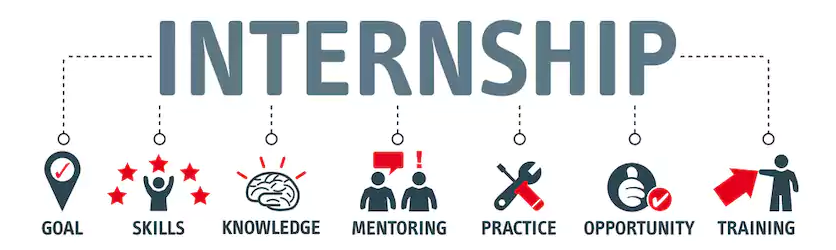
\includegraphics[width=\textwidth, keepaspectratio]{internship-businessstudent-com.png}
\centering
\caption{Caratteristiche dell'attività di tirocinio.} 
\source{\href{https://www.businessstudent.com/}{BusinessStudent.com}}
\label{fig:internship}
\end{figure}

%%%%%%%%%%%%%%%%%%%%%%%%%%%%%%%%%%%%%%%%%%%%%%%%%%%%%%%%%%%%%%%%%%%%%%%%%%%%%%%%%%%%%%%%%%%
\subsection{Presentazione dei progetti}
%descrizione generale dei progetti: \\
%- le idee che stanno dietro a questi\\
%- peculiarità\\
%- differenze con la concorrenza\\
Durante la mia attività di stage in \AD{} ho avuto modo di lavorare su due progetti: \textbf{DigitalSnapshots} e \textbf{AWMS}.\\
Entrambi i prodotti si basano su un'architettura di tipo \textit{\acrshort{saas}}.
I vantaggi di questa struttura sono molteplici: 
\begin{itemize}
\item \textbf{Accesso ad applicazioni sofisticate:} l'utilizzatore finale infatti non dovrà acquistare, installare, aggiornare o gestire nessun tipo di \textit{hardware}, \textit{middleware} o \textit{software};
\item \textbf{Pagamento solo per le risorse utilizzate:} l'architettura \textit{\acrshort{saas}} verticale è infatti molto modulare, e consente di fatturare solamente i servizi realmente utilizzati, tralasciando invece i servizi di cui non si usufruisce;
\item \textbf{Uso di software \markg{\gls{client}} gratuito:} essendo una soluzione completamente gestita, non vi è il bisogno di installare \gls{client} o applicazioni nel PC dell'utilizzatore. \`E necessario solamente un computer con un \textit{web browser} installato per poter accedere ai servizi erogati;
\item \textbf{Accesso ai dati da qualunque luogo:} con i dati archiviati nel \textit{\gls{cloud}}, gli utenti possono accedere alle informazioni da qualsiasi dispositivo connesso ad internet. Il \textit{\gls{cloud}} inoltre consente di non perdere i dati in caso di problemi al dispositivo fisico, garantendo così il recupero di tutte le informazioni con facilità.
\end{itemize}

\begin{figure}[h]
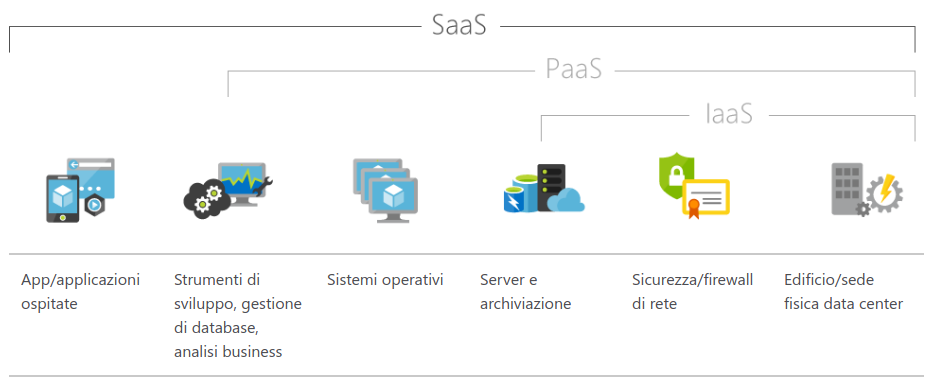
\includegraphics[width=\textwidth, keepaspectratio]{saas-microsoft.png}
\centering
\caption{Struttura di un'architettura \textit{\acrshort{saas}}.} 
\source{\href{https://www.azure.microsoft.com/}{Microsoft.com}}
\label{fig:saas-microsoft}
\end{figure}

DigitalSnapshots nasce dall'idea di fornire ai manager aziendali, uno strumento che facilitasse la gestione delle attività in corso nei vari stabilimenti. Esso permette all'utente di visualizzare tutte le attività in un'unica schermata, rendendo così più semplice il confronto e la valutazione. 
L'attività di stage a me proposta consisteva nel realizzare un modulo di analisi delle attività inserite, con la possibilità di filtraggio dei dati da analizzare, di selezione della tipologia di grafico da visualizzare, e di affiancamento di più grafici, così da rendere più efficaci i confronti effettuati. \\
%%%%%%%%%%%%%%%%%%%%%%%%%%%%%%%%%%%%%%%%%%%%%%%%%%%%%%%%%%%%%%%%%%%%%%%%%%%%%%%%%%%%%%%%%%%
L'idea che sta alla base di AWMS, invece, consiste nel fornire uno strumento per la gestione della manodopera all'interno degli stabilimenti produttivi delle aziende.
Questo significa inserire la persona giusta, nella postazione giusta, al momento giusto, così da massimizzare l'efficienza del reparto e migliorare la qualità del lavoro.
Questa piattaforma è innovativa in quanto sviluppata ponendo l'attenzione sulle persone anziché sui mezzi di produzione. Per effettuare la pianificazione quotidiana, infatti, l'algoritmo interno di AWMS terrà conto sia delle abilità di ogni persona disponibile, visitando lo storico delle mansioni svolte in passato da quest'ultime e controllando se siano in possesso delle certificazioni adeguate per svolgere l'attività che si sta andando a pianificare (si pensi ad esempio all'attività di carrellista, che necessita di un'apposita certificazione), che delle possibili disabilità o indisposizioni delle stesse.\\
In questo progetto, mi è stato proposto di realizzare un modulo per l'esportazione della pianificazione, sia in formato PDF, sia sotto forma di foglio elettronico.
%%%%%%%%%%%%%%%%%%%%%%%%%%%%%%%%%%%%%%%%%%%%%%%%%%%%%%%%%%%%%%%%%%%%%%%%%%%%%%%%%%%%%%%%%%%
\begin{figure}[h]
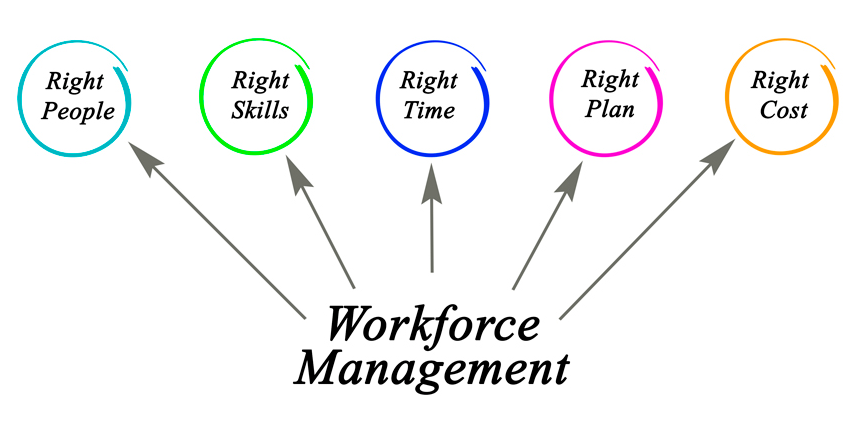
\includegraphics[width=\textwidth, keepaspectratio]{workforce-management.png}
\centering
\caption{Concetti di \textit{Workforce Management}.} 
\source{\href{https://www.replgroup.com/}{Replgroup.com}}
\label{fig:workforce-management}
\end{figure}

\subsection{Aspettative aziendali}
\label{subsec:aspettative-aziendali}
%definizione e classificazione degli obiettivi da raggiungere
Presentati i progetti, si è passati alla fase di definizione dei traguardi da raggiungere durante lo stage.
Il team di sviluppo ha deciso di suddividere questi obiettivi in due categorie: gli \textbf{obiettivi minimi} si riferiscono a dei compiti il cui completamento risulta essere indispensabile per l'avanzamento del progetto, gli \textbf{obiettivi opzionali} invece, fanno riferimento a delle caratteristiche del prodotto di importanza minore e quindi il loro soddisfacimento non è stato considerato obbligatorio.
Per ogni progetto, è stato assegnato a ciascun obiettivo un codice identificativo nel formato \textbf{O[tipo][numero]}, dove "tipo" assume il valore dell'iniziale della tipologia di obiettivo in considerazione, mentre con "numero" si intende il numero sequenziale di obiettivo di una determinata tipologia (ad esempio, il secondo obiettivo opzionale avrà la sigla OO2, mentre il primo obiettivo minimo sarà siglato OM1). \\
Di seguito, il riepilogo degli obiettivi che mi sono stati assegnati, ripartiti tra i vari progetti.
\subsubsection*{DigitalSnapshots}
\begin{center}
	\renewcommand{\arraystretch}{1.5}
	\rowcolors{2}{}{row}
	\begin{longtable}{ | p{0.1\linewidth} | p{0.9\linewidth} |}	 
		\hline   
	    \rowcolor{header}\textbf{Codice}&\textbf{Descrizione}\\
		\hline    	
    	OM1 & Ristrutturazione della base di dati MySQL e della parte Model di CakePHP \\
    	OM2 & Realizzazione moduli \markg{\acrshort{api}} e logica \\
    	OM3 & Creazione interfaccia utente del cruscotto delle analisi \\
    	OM4 & Stesura della documentazione su quanto realizzato \\
    	OO1 & Realizzazione di un modulo \textit{wizard} per la configurazione rapida del prodotto \\
    	OO2 & Implementazione di una gerarchia di utenti, con livelli di privilegi differenti \\
    	\hline
		\rowcolor{white}    	
    	\caption{Riepilogo obiettivi per il progetto DigitalSnapshots.}
	\end{longtable}
	\label{tab:obiettivi-digitalsnapshots}
\end{center}

\subsubsection*{AWMS}
\begin{center}
	\renewcommand{\arraystretch}{1.5}
	\rowcolors{2}{}{row}
	\begin{longtable}{ | p{0.1\linewidth} | p{0.9\linewidth} | }	 
		\hline   
	    \rowcolor{header}\textbf{Codice}&\textbf{Descrizione}\\
		\hline   	
    	OM1 & Implementazione dei dati necessari nel database PostgreSQL e nella parte Model di CakePHP \\
    	OM2 & Realizzazione moduli \acrshort{api} e logica \\
    	OM3 & Creazione interfaccia utente per la selezione della tipologia e delle opzioni di stampa \\
    	OM4 & Stesura della documentazione su quanto realizzato \\
    	OO1 & Realizzazione di un modulo per la configurazione dei ruoli degli utenti \\
    	OO2 & Implementazione di un migliore algoritmo di \textit{\gls{machine learning}} per la pianificazione intelligente della forza lavoro a disposizione \\
    	\hline
    	\rowcolor{white}
    	\caption{Riepilogo obiettivi per il progetto AWMS.}
	\end{longtable}
	\label{tab:obiettivi-AWMS}
\end{center}

\section{Vincoli}
\subsection{Vincoli temporali}
\label{subsec:vincoli-temporali}
%ore di lavoro complessive, scadenze sprint e scadenze di progetto

La durata complessiva dell'attività di stage è stata di 304 ore, distribuite, in accordo con il tutor aziendale, nell'arco di 8 settimane, ognuna delle quali aveva un monte orario di circa 40 ore. \\
L'orario lavorativo stabilito corrisponde all'orario di lavoro aziendale: dal Lunedì al Venerdì, dalle ore 9:00 alle 18:00.\\
Oltre a questo vincolo del monte orario, mi sono trovato a toccare con mano la pianificazione Scrum: all'inizio di ogni Sprint, infatti, ho pianificato le attività da portare a termine entro le successive due settimane, durata di ogni singolo Sprint.\\
Il progetto DigitalSnapshots inoltre, aveva una scadenza di consegna al cliente che combaciava con la fine del secondo Sprint, per cui il ritmo lavorativo è stato abbastanza elevato per non eccedere tale data.

\begin{figure}[h]
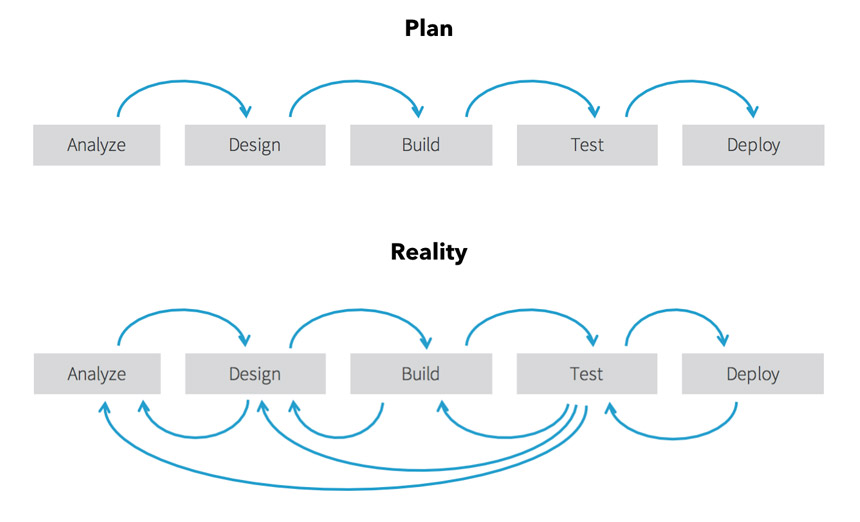
\includegraphics[width=\textwidth , keepaspectratio]{plan-vs-reality.jpg}
\centering
\caption{Rischi di pianificazione nell'attività di codifica.} 
\source{\href{https://www.devbridge.com/}{Devbridge.com}}
\label{fig:plan-vs-reality}
\end{figure}

\subsection{Vincoli metodologici}
\label{subsec:vincoli-metodologici}
%- monday meeting\\
%- interazione diretta con il cliente\\
%- scrum\\
%- Vincoli metodologici personali
Al mio arrivo in azienda, il progetto già presentava un'architettura e una metodologia di lavoro consolidate.
Data la mia poca esperienza con il \textit{\gls{framework}} Scrum, in accordo unanime tra tutto il team, abbiamo deciso di mantenere la durata degli Sprint pari a due settimane lavorative, ma di inserire a metà di questo lasso di tempo una riunione che aveva la funzione di monitorare l'andamento dello sviluppo e di rilevarne eventuali criticità. I \textit{meeting} di \textit{Sprint Review} erano spesso presenziati anche dal comparto tecnico o dalle persone di riferimento delle aziende \textit{stakeholder}, così da avere un \textit{\gls{feedback}} pressoché istantaneo su quanto fatto fino a quel momento.
A questi inoltre, si aggiunge la politica aziendale del \textit{Monday Meeting}, ovvero una assemblea, effettuata ogni due Lunedì, nel corso del quale si aggiornano i colleghi sull'andamento dei progetti in corso.\\
Nonostante avessi carta bianca sulla modalità di sviluppo del codice, mi sono posto dei vincoli da rispettare, affinchè l'attività risultasse il più efficiente ed efficace possibile.\\
Innanzitutto, ho scelto di seguire un approccio di sviluppo differente da quello classico, ovvero il \markg{\textit{\acrshort{tdd}}}. Acronimo di \textit{Test Driven Development}, consiste nel rovesciare il normale metodo di programmazione, in cui prima si codifica e poi si effettuano i test, obbligando così lo sviluppatore a scrivere il codice in base ai test che sono stati realizzati in precedenza.
In secondo luogo, ho configurato una \textit{pipeline} per la \markg{\textit{\gls{continuous integration}}} che eseguisse in maniera automatica i test precedentemente codificati e che caricasse nella \textit{repository} di lavoro, il codice da me realizzato.
\begin{figure}[h]
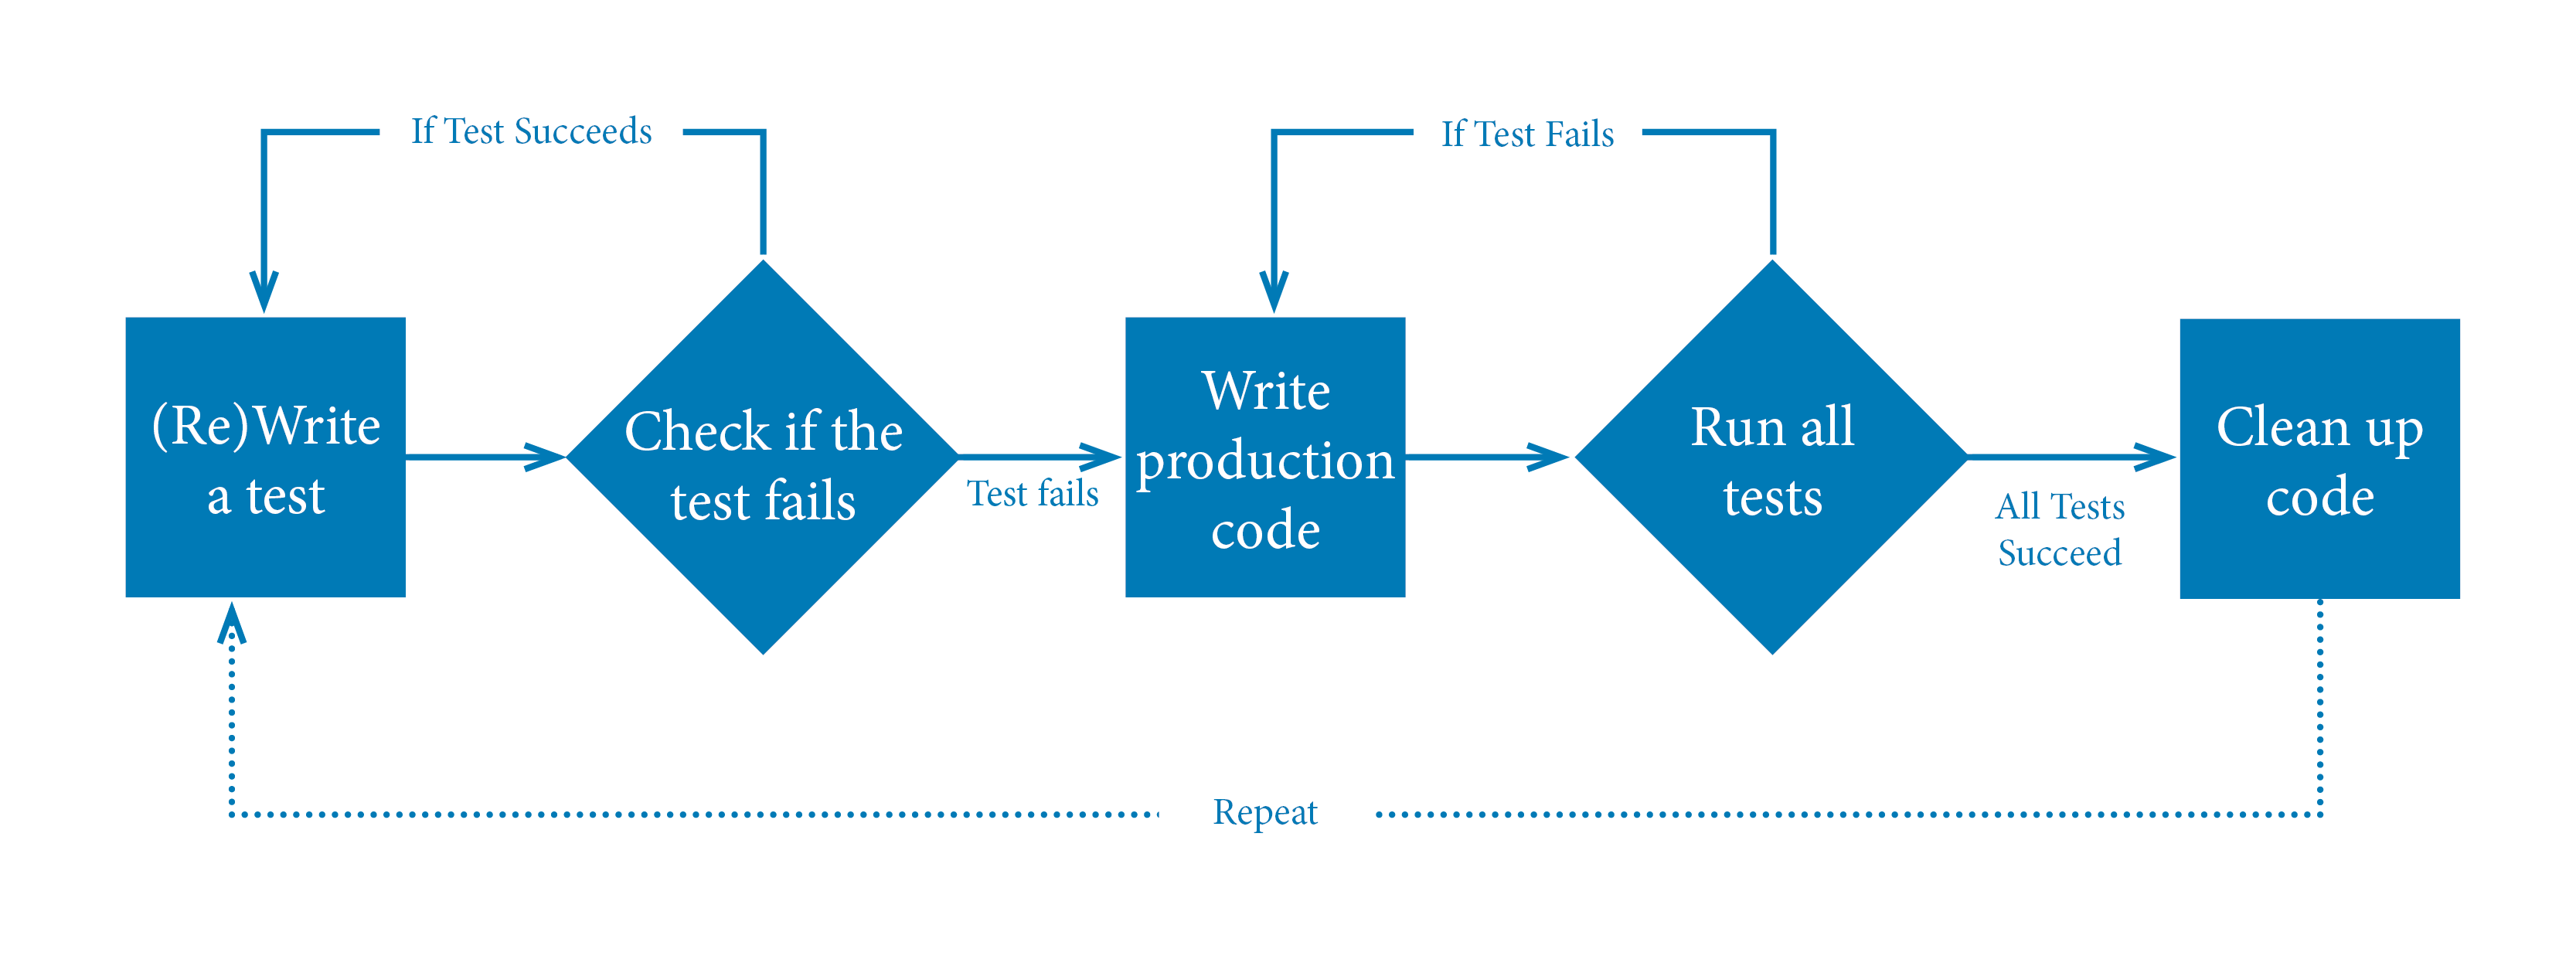
\includegraphics[width=\textwidth , keepaspectratio]{TestDrivenDevelopment.png}
\centering
\caption{Test Driven Development.} 
\source{\href{https://www.andplus.com/}{Andplus.com}}
\label{fig:tdd}
\end{figure}
%%%%%%%%%%%%%%%%%%%%%%%%%%%%%%%%%%%%%%%%%%%%%%%%%%%%%%%%%%%%%%%%%%%%%%%%%%%%%%%%%%%%%%%%%%%
\subsection{Vincoli tecnologici}
%stack tecnologico definito in avvio di progetto 

Per la realizzazione dei due progetti di stage, ho utilizzato due \textit{stack} tecnologici molto simili, ma per certi aspetti radicalmente differenti.\\
Il progetto AWMS si basa su tecnologie ampiamente utilizzate in azienda: 
\begin{itemize}
\item \textbf{PostgreSQL:} database relazionale, compatibile con il paradigma SQL, che consente all'utente di immagazzinare dati anche in formato Json, rendendo di fatto il contenuto delle tabelle molto più dinamico;
\item \textbf{CakePHP:} \textit{\gls{framework}} che consente lo sviluppo rapido di applicazioni web con architettura MVC. Grazie alla sua funzione di \markg{\textit{\acrshort{orm}}}, permette di effettuare operazioni sulle tabelle trattando quest'ultime come oggetti derivanti dal paradigma \markg{\textit{\acrshort{oop}}};
\item \textbf{Angular2+:} \textit{\gls{framework}} per lo sviluppo di applicazioni web \textit{single-page}.
\end{itemize}
DigitalSnapshots invece si differenzia da AWMS in quanto sostituisce \textbf{MySQL} a \textit{PostgreSQL} e \textbf{AngularJS} ad \textit{Angular2+}.\\
Questa differenza di comparto tecnico è giustificata dal fatto che, mentre AWMS verrà seguito da \AD{} (nello specifico, da \textbf{I4.0Saas} dal 2020) per tutto il suo ciclo di vita, DigitalSnapshots avrà un destino differente: le fasi di progettazione e sviluppo sono a carico di \AD{}, mentre la fase di manutenzione del codice sarà eseguita dal reparto tecnico di Electrolux, committente del progetto.\\
Dai vincoli metodologici personali, deriva l'utilizzo dei \textit{\gls{framework}} \textit{Jenkins}, per l'implementazione della \textit{continous integration}, e \textit{PHPUnit} e \textit{Jasmine} per l'esecuzione automatica dei test d'unità ed integrazione, rispettivamente per i linguaggi di programmazione PHP e Typescript.
\section{Aspettative personali}
%- come ho conosciuto AD\\
%- perchè AD?\\
%- aspettative sul lavorare in una startup, imparare il way of working\\
Durante l'ultimo anno del mio percorso accademico, ho avuto l'opportunità di partecipare a \textit{Stage-IT}, un evento organizzato da Assindustria Venetocentro in collaborazione con l'Università di Padova, con lo scopo di fornire un punto di contatto tra gli studenti e le aziende del settore informatico presenti nel territorio.
\`E proprio durante questo incontro che ho conosciuto \AD , e subito sono rimasto intrigato dalla sua dinamicità e propensione all'innovazione, nonché dai progetti ambiziosi e dai valori aziendali nei quali mi identifico.\\
\begin{figure}[h!]

\includegraphics[width=\textwidth]{startup.jpg}
\centering
\caption{Le molte sfaccettature delle start-up.} 
\source{\href{http://orizzonti.tv/}{Orizzonti.tv}}
\label{fig:startup}
\end{figure}

Le mie aspettative riguardo a questa attività di stage potevano essere riassunte in tre punti fondamentali:
\begin{itemize}
\item Innanzitutto, vedevo questo tirocinio come un banco di prova su cui testare le conoscenze acquisite durante il percorso universitario e la mia capacità di apprendimento di tecnologie a me perlopiù sconosciute;
\item In secondo luogo, ero desideroso di collaborare con aziende dal marchio rinomato;
\item Infine, ma non per questo meno importante, desideravo imparare il \markg{\textit{\gls{way of working}}} da persone con esperienza nel settore dell'\textit{\acrshort{it}}, perchè credo che conoscere gli strumenti e saperli utilizzare al meglio sia fondamentale per uno sviluppatore, specie se inesperto.
\end{itemize}
Ho scelto \AD{} come sede nella quale svolgere l'attività di stage curriculare in quanto, oltre ad avere il potenziale per soddisfare le mie aspettative, mi avrebbe permesso di rendermi utile non solamente nell'attività di progettazione e codifica, ma anche nell'attività di analisi funzionale: prima di intraprendere la carriera accademica infatti, ho avuto modo di lavorare per diversi anni all'interno del settore manifatturiero, sviluppando così una discreta esperienza nella gestione della workforce aziendale.
%%%%%%%%%%%%%%%%%%%%%%%%%%%%%%%%%%%%%%%%%%%%%%%%%%%%%%%%%%%%%%%%%%%%%%%%%%%%%%%%%%%%%%%%%%%